% ============================================================
% 数电实验报告 — 实验五：基于 ROM 的波形发生与字符显示系统
% ============================================================

\documentclass[12pt]{ctexart}

% --- 宏包 ---
\usepackage{graphicx}
\usepackage{amsmath}
\usepackage{xcolor}
\usepackage{float}
\usepackage{booktabs}
\usepackage{siunitx}
\usepackage{fancyhdr}
\usepackage{caption}
\usepackage{subcaption}
\usepackage{hyperref}
\usepackage{makecell}
\usepackage{enumitem}
\usepackage[outputdir=build]{minted}

\sisetup{per-mode=symbol}

\graphicspath{{./figures/}{../figures/}}

\usepackage[left=2.5cm, right=2.5cm, top=2.5cm, bottom=2.5cm]{geometry}

\setlength{\jot}{6pt}
\setlength{\headheight}{15pt}
\linespread{1.5}
\setlist{nosep}

% --- VHDL 代码样式 ---
\setminted[vhdl]{
    fontsize=\small,
    frame=single,
    linenos,
    breaklines,
    tabsize=4,
    numbersep=8pt,
    xleftmargin=2em
}

% --- 页眉页脚 ---
\pagestyle{fancy}
\fancyhead[C]{数字电子技术实验}
\fancyfoot[C]{\thepage}

\begin{document}

% ==================== 封面 ====================
\thispagestyle{empty}

\begin{figure}[t]
    \centering
    
\includegraphics[width=13cm]{logo1.png}
\end{figure}

\vspace*{\fill}
    \begin{center}
        \Huge\textbf{数字电子技术基础}

        \vspace{0.3cm}
        \Huge\textbf{实验报告}

        \vspace{1cm}
        \LARGE\textbf{实验五：基于 ROM 的波形发生与字符显示系统}
    \end{center}
\vspace*{\fill}

\begin{table}[H]
    \centering
    \large
    \begin{tabular}{ll}
    \toprule
    \textbf{课程:} & 数字电子技术实验 \\
    \textbf{组员1:} & 郭浩然 2024303980 \\
    \textbf{组员2:} & 庞铭洋 2024302539 \\
    \textbf{组号:} & 15 \\
    \textbf{时间:} & \today \\
    \bottomrule
    \end{tabular}
\end{table}

\newpage

% ==================== 正文 ====================

\section{实验目的}

\begin{enumerate}
    \item 掌握只读存储器 ROM 在数字系统中的应用，熟悉 Quartus II 中 ROM IP 核 \texttt{altsyncram} 的配置流程和 \texttt{.mif} 文件的数据初始化方法。
    \item 理解用计数器扫描 ROM 地址来顺序输出数据的设计思路，掌握用 ROM 查表产生正弦波、显示字符序列的原理。
    \item 学会把分频器、计数器、ROM、译码器组合成一个系统，先用 VHDL 编写各功能模块，再用原理图把它们连接起来，完成混合设计。
    \item 学会用拨码开关和门电路实现模式切换，并在 DE0 开发板上用 LED 和七段数码管验证结果。
\end{enumerate}

\section{实验要求}

本次实验的要求以现场给出的实验内容为准，具体如下：

\begin{enumerate}
    \item \textbf{要求 1}：配置一块宽度为 8 位的 ROM，在其中存储 512 个地址的正弦波数据。以系统时钟作为计数器的计数脉冲，用 74161 一类的计数器模块、或用硬件描述语言编写的计数模块，让其输出依次扫描 ROM 的地址端，把 ROM 中保存的数据按 1\,Hz 的频率输出，通过 DE0 开发板上的 8 位 LED 灯查看并验证。
    \item \textbf{要求 2}：配置一块存储学号的 ROM，学号内容取同学 A 的后 4 位学号，接上 F、L、E、P，再接同学 B 的后 3 位学号。用计数器的输出依次扫描 ROM 的地址端，把数据按 1\,Hz 的频率输出，通过 DE0 开发板上的 1 个七段数码管查看并验证。
    \item \textbf{要求 3}：要求 2 与要求 1 通过控制开关切换。
\end{enumerate}

本组两名同学中，同学 A 庞铭洋的学号为 2024302539，同学 B 郭浩然的学号为 2024303980。按要求 2 的规则，同学 A 的后 4 位是 \texttt{2539}，同学 B 的后 3 位是 \texttt{980}，中间插入 F、L、E、P，因此本组要在七段数码管上循环显示的字符序列为 \texttt{2539FLEP980}，一共 11 个字符。

\section{实验设备}

\begin{itemize}
    \item Quartus II 开发软件，含 MegaWizard Plug-In Manager 和 ROM IP 核
    \item DE0 开发板，FPGA 型号为 Cyclone V 5CEBA4F23C7
    \item USB-Blaster 下载线及计算机
    \item 板载 50\,MHz 晶振、拨码开关、8 个红色 LED 灯 LEDR 和七段数码管 HEX0
\end{itemize}

\section{实验原理}

\subsection{ROM 存储器原理}

只读存储器 ROM 是一种非易失性存储器，写入之后内容只能读出，不能在运行过程中修改。它的工作方式就是查表：把地址作为索引送进去，ROM 就把该地址上事先存好的数据读出来，即
\[
    \mathrm{data\_out} = \mathrm{ROM}[\mathrm{addr}].
\]

本实验的 ROM 用 Quartus II 自带的 \texttt{altsyncram} IP 核实现，在 MegaWizard Plug-In Manager 里可以直接设定数据宽度、存储深度和初始化文件 \texttt{.mif}，综合后由 FPGA 内部的 M10K 嵌入式存储块承担。本实验用到两块 ROM：

\begin{itemize}
    \item \textbf{正弦波 ROM} \texttt{sinrom}：数据宽度 8 位，深度 512 字，地址位宽取 9 位，对应 $2^9 = 512$ 个地址；初始化文件是 \texttt{dds\_512x8b\_wave.mif}，存的是一个完整周期正弦波的 512 点等间隔采样，数值在 $0\sim255$ 之间，零点偏置约为 128。
    \item \textbf{学号字符 ROM} \texttt{xuehaoHOPE}：数据宽度 4 位，深度 32 字，地址位宽 5 位；初始化文件是 \texttt{Mif1.mif}，地址 $0\sim10$ 这 11 个单元存放待显示字符的 4 位编码索引，其余地址填 0。
\end{itemize}

\subsection{计数器扫描与查表式波形发生原理}

ROM 只负责把地址映射成数据。要让数据按时间顺序自动输出，还需要一个地址计数器不断地把 ROM 的地址从头扫到尾。计数器在扫描时钟驱动下从 0 加到最大地址再归零，ROM 输出端就按存储顺序循环送出各个采样点，存进去的波形或字符序列也就在输出端重建出来。直接数字频率合成 DDS 产生任意波形，依靠的正是这种存采样、扫地址的方法。

\begin{itemize}
    \item 正弦波模式用一个模 512 计数器产生 $0\sim511$ 的 9 位地址，逐点扫过正弦波 ROM，把 512 个采样值依次送到 8 位 LED 上，LED 的亮灭组合就反映出正弦幅值的周期变化。
    \item 学号模式用一个模 11 计数器产生 $0\sim10$ 的地址，循环扫描学号 ROM 的 11 个有效单元，输出经七段译码后在数码管上循环显示这 11 个字符。
\end{itemize}

\subsection{分频原理}

DE0 开发板的系统时钟是 50\,MHz，若直接用它作扫描时钟，LED 和数码管刷新太快，肉眼无法分辨，所以要先分频，把扫描频率降到 1\,Hz 上下。分频就是对高频时钟计数：设输入频率为 $f_{\text{clk}}$、期望输出频率为 $f_{\text{out}}$，要得到占空比 50\% 的方波，半周期需要的计数值为
\[
    N = \frac{f_{\text{clk}}}{2 \times f_{\text{out}}}.
\]
把 50\,MHz 分到 1\,Hz 时，$N = 50{,}000{,}000 / 2 = 25{,}000{,}000$。顶层把这一步交给 \texttt{lpm\_counter0} 完成，它是一个 26 位的 LPM 计数器 IP，对系统时钟分频后取出一路低速脉冲，作为约 1\,Hz 量级的扫描时钟去驱动后面的电路。

\subsection{模式切换原理}

两种模式共用同一路分频后的扫描时钟，由拨码开关 \texttt{switch} 决定让哪条数据通路工作。顶层用一个反相器和两个二输入与门，把扫描时钟分别门控到两条通路上，逻辑见表~\ref{tab:mode}。哪条通路被关闭，它的计数器就停止计数，对应 ROM 的寄存输出保持原值，两条通路互不影响。两个计数器的复位端 \texttt{RST} 都接高电平 VCC，也就是始终不复位、保持正常计数。

\begin{table}[H]
    \centering
    \caption{模式切换功能对照表}
    \label{tab:mode}
    \begin{tabular}{cccc}
        \toprule
        \textbf{switch} & \textbf{工作模式} & \textbf{扫描时钟使能的通路} & \textbf{现象} \\
        \midrule
        0 & 正弦波模式   & \texttt{Vhd1}+\texttt{sinrom}     & 8 位 LED 显示正弦采样；数码管保持不变 \\
        1 & 学号序列模式 & \texttt{time2}+\texttt{xuehaoHOPE} & 数码管循环显示学号字符；LED 保持 0 \\
        \bottomrule
    \end{tabular}
\end{table}

\subsection{七段数码管译码原理}

学号 ROM 送出的是 4 位编码索引，要先经七段译码器 \texttt{bin2seg} 转换成 7 位段选信号才能驱动数码管。DE0 板上的七段数码管是共阳极结构，段选信号低电平有效，即某段给 0 点亮、给 1 熄灭。编码索引与显示字符的对应关系见表~\ref{tab:bin2seg}。

\begin{table}[H]
    \centering
    \caption{\texttt{bin2seg} 七段译码真值表，段序 abcdefg、低电平有效}
    \label{tab:bin2seg}
    \begin{tabular}{ccc}
        \toprule
        \textbf{bin\_input[3:0]} & \textbf{seg\_output[6:0]} & \textbf{显示字符} \\
        \midrule
        0000 & 0010010 & 5 \\
        0001 & 0110000 & 3 \\
        0010 & 0010000 & 9 \\
        0011 & 0001110 & F \\
        0100 & 1000111 & L \\
        0101 & 0000110 & E \\
        0110 & 0001100 & P \\
        0111 & 0010000 & 9 \\
        1000 & 0000000 & 8 \\
        1001 & 1000000 & 0 \\
        1010 & 0100100 & 2 \\
        其他 & 1111111 & 全灭 \\
        \bottomrule
    \end{tabular}
\end{table}

\section{实验内容}

本系统把 VHDL 文本设计和原理图设计结合起来：各功能子模块用 VHDL 编写，编译后生成原理图符号，再在顶层原理图中调用、连线，拼成完整系统。整个软件流程是：建立工程，用 MegaWizard 配置两块 ROM IP 核，编写各子模块 VHDL 代码并生成符号，绘制顶层原理图，编译，波形仿真，引脚分配，最后下载到开发板验证。

\subsection{建立工程与配置 ROM IP 核}

打开 Quartus II，用 \textbf{File $\rightarrow$ New Project Wizard} 新建工程，器件选 DE0 开发板对应的 Cyclone V \texttt{5CEBA4F23C7}。随后打开 \textbf{Tools $\rightarrow$ MegaWizard Plug-In Manager}，按 \texttt{ROM: 1-PORT} 类型配置两块 ROM IP 核：

\begin{enumerate}
    \item \textbf{正弦波 ROM \texttt{sinrom}}：输出位宽设为 8 位，深度设为 512 字，地址 9 位，勾选用 \texttt{.mif} 文件初始化并指定 \texttt{dds\_512x8b\_wave.mif}。这个 \texttt{.mif} 里的 512 点正弦采样不是手工填的，而是用波形转换工具 \texttt{WaveToMif} 从一个周期的正弦波生成，幅值范围 $0\sim255$。前几个采样值列在表~\ref{tab:sinmif}。
    \item \textbf{学号字符 ROM \texttt{xuehaoHOPE}}：输出位宽设为 4 位，深度设为 32 字，用 \texttt{Mif1.mif} 初始化。\texttt{Mif1.mif} 的内容以及经 \texttt{bin2seg} 译码后显示的字符见表~\ref{tab:xuehaomif}。
\end{enumerate}

\begin{table}[H]
    \centering
    \caption{正弦波 ROM 初始化文件 \texttt{dds\_512x8b\_wave.mif} 部分采样值}
    \label{tab:sinmif}
    \begin{tabular}{cccccccccc}
        \toprule
        地址 & 0 & 1 & 2 & 3 & 4 & 5 & 6 & 7 & $\cdots$ \\
        \midrule
        十进制数据 & 127 & 128 & 130 & 131 & 133 & 134 & 136 & 137 & $\cdots$ \\
        \bottomrule
    \end{tabular}
\end{table}

\begin{table}[H]
    \centering
    \caption{学号字符 ROM 初始化文件 \texttt{Mif1.mif} 内容与显示映射}
    \label{tab:xuehaomif}
    \begin{tabular}{cccc}
        \toprule
        \textbf{ROM 地址} & \textbf{存储的 4 位编码} & \textbf{经 \texttt{bin2seg} 译码} & \textbf{显示字符} \\
        \midrule
        0  & 1010 & 0100100 & 2 \\
        1  & 0000 & 0010010 & 5 \\
        2  & 0001 & 0110000 & 3 \\
        3  & 0010 & 0010000 & 9 \\
        4  & 0011 & 0001110 & F \\
        5  & 0100 & 1000111 & L \\
        6  & 0101 & 0000110 & E \\
        7  & 0110 & 0001100 & P \\
        8  & 0111 & 0010000 & 9 \\
        9  & 1000 & 0000000 & 8 \\
        10 & 1001 & 1000000 & 0 \\
        11--31 & 0000 & --- & 未使用 \\
        \bottomrule
    \end{tabular}
\end{table}

把地址 $0\sim10$ 顺序读出后，数码管上正好显示 \texttt{2539FLEP980}，与要求 2 一致。

\subsection{编写各子模块 VHDL 代码}

\subsubsection{模 512 地址计数器 Vhd1}

\texttt{Vhd1} 负责产生正弦波 ROM 的 9 位地址。扫描时钟每来一个上升沿就计数加 1，数到 511 后归零，同时给出一个进位脉冲 \texttt{COUT}，这样循环扫完 512 个地址；\texttt{RST} 为低电平时异步清零。

\begin{minted}{vhdl}
LIBRARY IEEE;
USE IEEE.STD_LOGIC_1164.ALL;
USE IEEE.STD_LOGIC_UNSIGNED.ALL;
ENTITY Vhd1 IS
    PORT ( clk,RST : IN  STD_LOGIC;
           DOUT    : OUT STD_LOGIC_VECTOR (8 DOWNTO 0);  -- 9位计数
           COUT    : OUT STD_LOGIC);                      -- 进位位
END Vhd1;
ARCHITECTURE fwm OF Vhd1 IS
    SIGNAL Q1 : STD_LOGIC_VECTOR (8 DOWNTO 0);
BEGIN
PROCESS(clk,RST)
BEGIN
    IF RST = '0' THEN
        Q1 <= (OTHERS => '0'); COUT <= '0';
    ELSIF clk'EVENT AND clk = '1' THEN
        Q1 <= Q1 + 1;
        COUT <= '0';
        IF Q1 >= "111111111" THEN          -- 计满 511 归零
            Q1 <= (OTHERS => '0'); COUT <= '1';
        END IF;
    END IF;
END PROCESS;
DOUT <= Q1;
END fwm;
\end{minted}
\captionof{listing}{模 512 地址计数器 Vhd1.vhd}
\label{lst:vhd1}

\subsubsection{模 11 地址计数器 time2}

\texttt{time2} 负责产生学号 ROM 的地址，计数范围 $0\sim10$，对应 11 个有效字符，数到 10 后下一拍归零，做成 11 进制循环计数。

\begin{minted}{vhdl}
LIBRARY IEEE;
USE IEEE.STD_LOGIC_1164.ALL;
USE IEEE.STD_LOGIC_UNSIGNED.ALL;
ENTITY time2 IS
    PORT ( clk,RST : IN  STD_LOGIC;
           DOUT    : OUT STD_LOGIC_VECTOR (4 DOWNTO 0);  -- 五位计数
           COUT    : OUT STD_LOGIC);                      -- 进位位
END time2;
ARCHITECTURE fwm OF time2 IS
    SIGNAL Q1 : STD_LOGIC_VECTOR (4 DOWNTO 0);
BEGIN
    PROCESS(clk,RST)
    BEGIN
        IF RST = '0' THEN
            Q1 <= (OTHERS => '0'); COUT <= '0';
        ELSIF clk'EVENT AND clk = '1' THEN
            Q1 <= Q1 + 1;
            COUT <= '0';
            IF Q1 >= "01010" THEN          -- 计到 10 归零
                Q1 <= (OTHERS => '0'); COUT <= '1';
            END IF;
        END IF;
    END PROCESS;
    DOUT <= Q1;
END fwm;
\end{minted}
\captionof{listing}{模 11 地址计数器 time2.vhd}
\label{lst:time2}

\subsubsection{七段数码管译码器 bin2seg}

\texttt{bin2seg} 接收学号 ROM 输出的 4 位编码，用 \texttt{case} 语句映射成共阳极七段码，低电平有效，实现表~\ref{tab:bin2seg} 中的字符显示。

\begin{minted}{vhdl}
library IEEE;
use IEEE.STD_LOGIC_1164.ALL;
entity bin2seg is
    Port ( bin_input  : in  STD_LOGIC_VECTOR(3 downto 0);  -- 4位二进制输入
           seg_output : out STD_LOGIC_VECTOR(6 downto 0)); -- 七段输出(abcdefg)
end bin2seg;
architecture Behavioral of bin2seg is
begin
    process(bin_input)
    begin
        case bin_input is                  -- 共阳极数码管段码（低电平有效）
            when "0000" => seg_output <= "0010010"; -- 5
            when "0001" => seg_output <= "0110000"; -- 3
            when "0010" => seg_output <= "0010000"; -- 9
            when "0011" => seg_output <= "0001110"; -- F
            when "0100" => seg_output <= "1000111"; -- L
            when "0101" => seg_output <= "0000110"; -- E
            when "0110" => seg_output <= "0001100"; -- P
            when "0111" => seg_output <= "0010000"; -- 9
            when "1000" => seg_output <= "0000000"; -- 8
            when "1001" => seg_output <= "1000000"; -- 0
            when "1010" => seg_output <= "0100100"; -- 2
            when others => seg_output <= "1111111"; -- 全灭
        end case;
    end process;
end Behavioral;
\end{minted}
\captionof{listing}{七段数码管译码器 bin2seg.vhd}
\label{lst:bin2seg}

分频功能由 \texttt{lpm\_counter0} 这个 26 位 LPM 计数器 IP 完成。把上面几个 VHDL 模块分别编译，再用 \textbf{File $\rightarrow$ Create/Update $\rightarrow$ Create Symbol Files for Current File} 各自生成 \texttt{.bsf} 符号，连同两块 ROM IP 的符号一起供顶层原理图调用。

\subsection{绘制顶层原理图}

新建一个 BDF 原理图作为顶层设计，把各模块符号放上去，按下面的关系连线，顶层原理图如图~\ref{fig:top}。

\begin{itemize}
    \item 输入有两个：\texttt{clk} 接板载 50\,MHz 系统时钟，\texttt{switch} 接模式选择拨码开关。
    \item \texttt{lpm\_counter0} 以 \texttt{clk} 为时钟，对系统时钟分频，得到低速扫描时钟。
    \item \texttt{switch} 经反相器取反后与扫描时钟相与，得到正弦波通路的时钟，驱动 \texttt{Vhd1} 和 \texttt{sinrom}；\texttt{switch} 不取反、直接与扫描时钟相与，得到学号通路的时钟，驱动 \texttt{time2} 和 \texttt{xuehaoHOPE}。两个计数器的 \texttt{RST} 都接 VCC，始终不复位。
    \item \texttt{Vhd1} 的 \texttt{DOUT[8..0]} 接 \texttt{sinrom} 的 \texttt{address[8..0]}，\texttt{sinrom} 的 \texttt{q[7..0]} 接 8 位输出 \texttt{led[7..0]}。
    \item \texttt{time2} 的 \texttt{DOUT[4..0]} 接 \texttt{xuehaoHOPE} 的 \texttt{address[4..0]}，\texttt{xuehaoHOPE} 的 \texttt{q[3..0]} 接 \texttt{bin2seg} 的 \texttt{bin\_input[3..0]}，译码输出 \texttt{seg\_output[6..0]} 拆分为 7 个段选输出 \texttt{A,b,c,d,e,f,g} 接七段数码管 HEX0。
\end{itemize}

\begin{figure}[H]
    \centering
    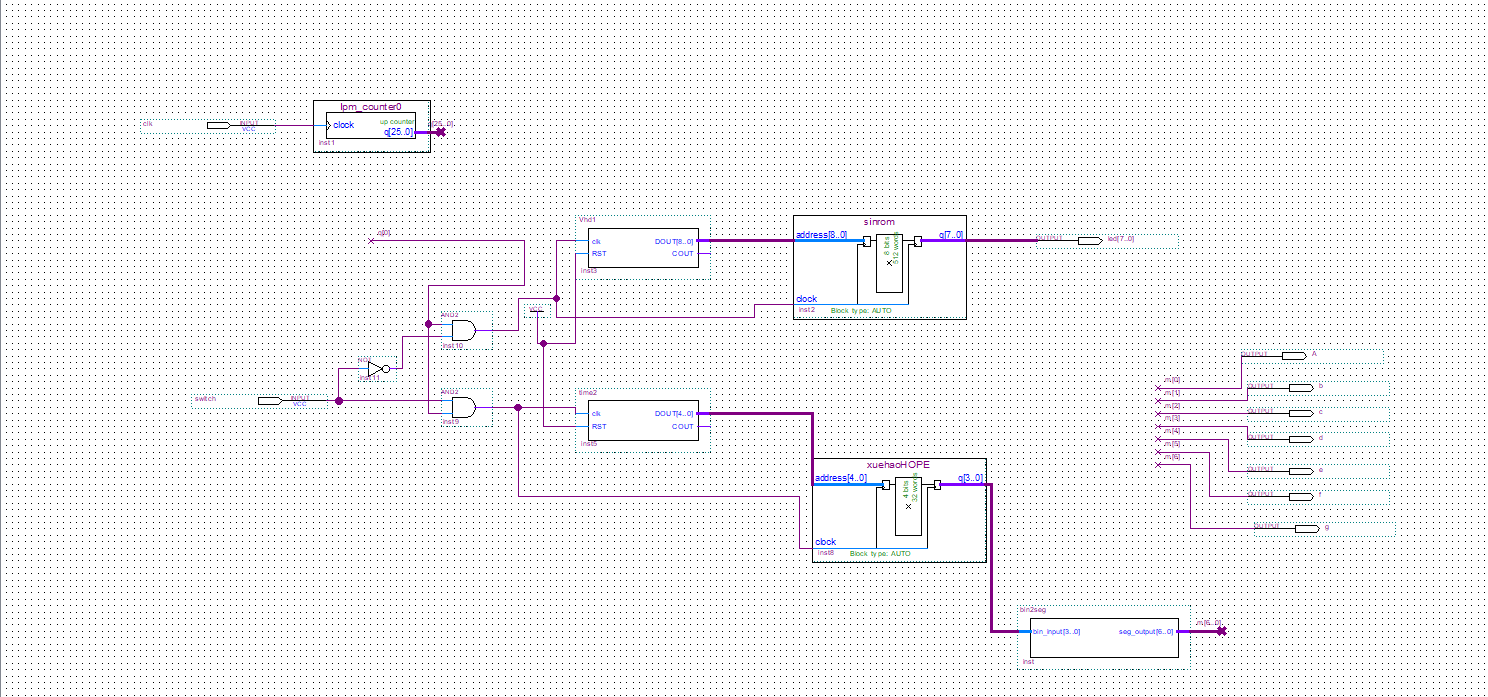
\includegraphics[width=0.98\textwidth]{电路图.png}
    \caption{基于 ROM 的波形发生与字符显示系统顶层原理图}
    \label{fig:top}
\end{figure}

\subsection{编译与波形仿真}

把 BDF 文件设成顶层实体，完整编译一遍。实际分频系数很大，若照真实时钟仿真要花很长时间，所以仿真时先把扫描时钟的分频比临时调小，让计数器快速扫完 ROM，在可接受的时间内把逻辑验证清楚；下载到开发板时再把分频比改回去，恢复约 1\,Hz 的实际扫描频率。

\subsubsection{正弦波模式仿真}

把 \texttt{switch} 置 0，新建波形文件，加入 \texttt{clk}、\texttt{switch}、\texttt{led[7..0]} 等信号运行功能仿真，结果如图~\ref{fig:sim1}。

\begin{figure}[H]
    \centering
    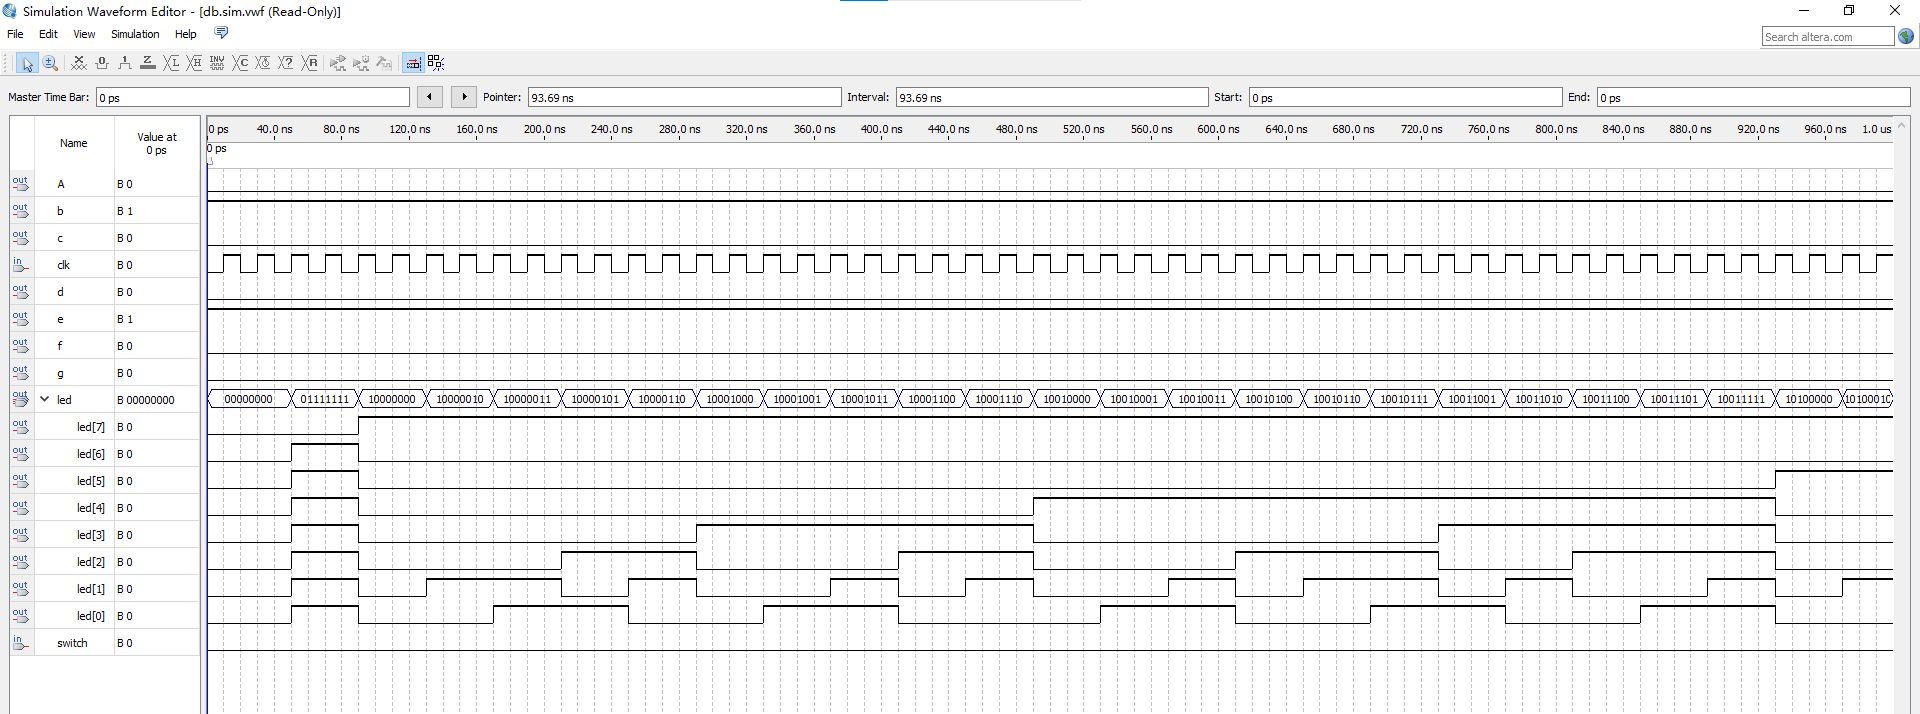
\includegraphics[width=0.98\textwidth]{任务1仿真.png}
    \caption{switch = 0 时的正弦波模式功能仿真波形}
    \label{fig:sim1}
\end{figure}

\texttt{switch} 一直保持低电平，系统处于正弦波输出模式。\texttt{led[7..0]} 从初值 \texttt{00000000} 起，随 \texttt{Vhd1} 的地址递增依次输出 \texttt{01111111}、\texttt{10000000}、\texttt{10000010}、\texttt{10000011}、\texttt{10000101}、\texttt{10000110} 等，换算成十进制就是 127、128、130、131、133、134，数值一路上升，与表~\ref{tab:sinmif} 中 \texttt{dds\_512x8b\_wave.mif} 预存的采样值逐一吻合，说明正弦波 ROM 的地址扫描和数据输出都正确。这时学号通路的时钟被关闭，数码管段选保持在地址 0 对应的字符 \texttt{2} 上不变。

\subsubsection{学号序列模式仿真}

把 \texttt{switch} 置 1，加入七段输出 \texttt{A,b,c,d,e,f,g} 和 \texttt{led} 等信号再运行一次仿真，结果如图~\ref{fig:sim2}。

\begin{figure}[H]
    \centering
    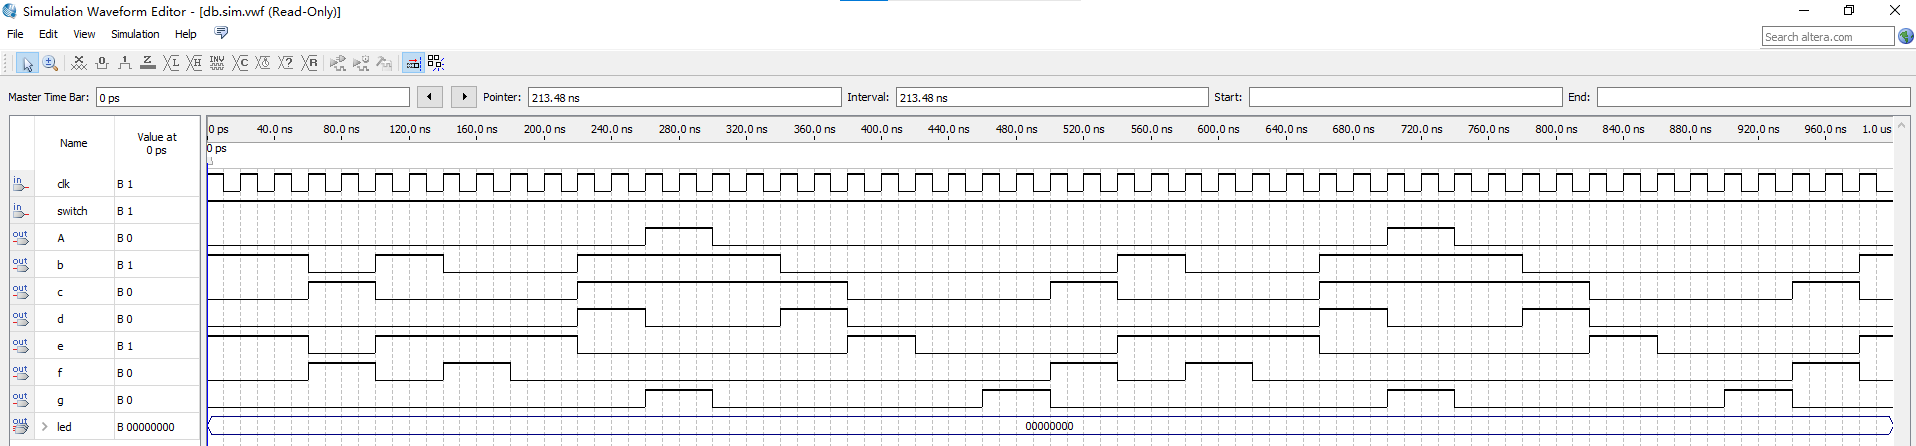
\includegraphics[width=0.98\textwidth]{任务2仿真.png}
    \caption{switch = 1 时的学号序列模式功能仿真波形}
    \label{fig:sim2}
\end{figure}

\texttt{switch} 一直保持高电平，系统处于学号序列输出模式。\texttt{time2} 的地址从 0 递增到 10 再归零循环，七段输出 \texttt{A,b,c,d,e,f,g} 随之变化，依次给出 \texttt{2539FLEP980} 各字符对应的段选码。例如地址为 0 时 \texttt{A,b,c,d,e,f,g} 为 \texttt{0100100}，对应字符 \texttt{2}，与表~\ref{tab:xuehaomif} 的映射完全一致。这时正弦波通路被关闭，\texttt{led[7..0]} 保持 \texttt{00000000} 不变。可见学号 ROM 的扫描和译码显示功能都正确。

\subsection{引脚分配与下载验证}

打开 Pin Planner，把各端口锁定到 DE0 开发板对应的硬件资源上，分配关系见表~\ref{tab:pins}。

\begin{table}[H]
    \centering
    \caption{引脚分配：端口与 DE0 板载资源的对应关系}
    \label{tab:pins}
    \begin{tabular}{ccl}
        \toprule
        \textbf{端口} & \textbf{方向} & \textbf{对应 DE0 硬件资源} \\
        \midrule
        clk               & 输入 & 板载 50\,MHz 系统时钟 CLOCK \\
        switch            & 输入 & 模式选择拨码开关 \\
        led[7..0]         & 输出 & 8 个红色 LED，LEDR7$\sim$LEDR0 \\
        A, b, c, d, e, f, g & 输出 & 七段数码管 HEX0 的 a$\sim$g 段 \\
        \bottomrule
    \end{tabular}
\end{table}

重新编译后，接上 USB-Blaster，用 JTAG 模式把 \texttt{.sof} 配置文件下载到 DE0 开发板进行硬件验证：

\begin{itemize}
    \item \texttt{switch} 拨到低电平时，系统进入正弦波模式，8 位 LED 以约 1\,Hz 的节奏依次刷新，亮灭组合呈现正弦幅值先增大后减小的周期变化，数码管显示保持不变。
    \item \texttt{switch} 拨到高电平时，系统进入学号序列模式，七段数码管 HEX0 以约 1\,Hz 的节奏循环显示 \texttt{2}、\texttt{5}、\texttt{3}、\texttt{9}、\texttt{F}、\texttt{L}、\texttt{E}、\texttt{P}、\texttt{9}、\texttt{8}、\texttt{0} 共 11 个字符，LED 全部熄灭。
    \item 拨动 \texttt{switch} 可在两种模式间实时切换，运行稳定，硬件现象与仿真一致。
\end{itemize}

\section{实验过程中的问题}

\begin{enumerate}
    \item \textbf{ROM 数据宽度的选择}。学号字符 ROM 第一次配置时数据宽度设大了，其实 11 个字符的编码索引只到 10，用 4 位就够。位宽偏大不影响功能，但多占了存储资源。后来用 MegaWizard 把数据宽度改成 4 位、深度取 32 字，占用就合理了。
    \item \textbf{\texttt{.mif} 文件要与 ROM 参数对上}。\texttt{.mif} 里的 \texttt{WIDTH}、\texttt{DEPTH} 必须与 ROM IP 的位宽、深度一致，地址和数据的基数 \texttt{ADDRESS\_RADIX}、\texttt{DATA\_RADIX} 也要写对，否则综合时会报错，提示初始化数据无法识别。正弦采样的 \texttt{.mif} 用 \texttt{WaveToMif} 工具从波形直接生成，省去了手工填写 512 个数据，也避免了填错。
    \item \textbf{仿真时间过长}。实际分频系数很大，分到 1\,Hz 要对 50\,MHz 计数 2500 万次，计数器跑完一整轮 ROM 扫描需要很久，仿真效率很低。办法是仿真时先把分频比调小，让计数器快速走完地址，短时间内就能验证逻辑；下载前再把分频比改回去，保证实际输出约 1\,Hz。
    \item \textbf{模式切换的实现方式}。要求 3 要两种模式能用开关切换。本设计没有在 ROM 的数据输出端做多路选择，而是用 \texttt{switch} 经反相器和与门门控两条通路的扫描时钟，只让选中那条的计数器走时钟、另一条冻结。这样实现简单，两条通路互不干扰；被冻结通路的 ROM 寄存输出保持原值，例如正弦通路停下时 LED 就保持在初始的 0。
\end{enumerate}

\section{心得体会}

\begin{enumerate}
    \item 这次实验让我把 ROM 在 FPGA 中的用法理解得更清楚。ROM 就是一张查找表，配上地址计数器顺序扫描，就能产生任意波形、循环显示字符序列。先把数据存好、再按地址取出来，DDS 这类技术依靠的正是这个思路。
    \item 配置 \texttt{altsyncram} ROM IP 核、编写 \texttt{.mif} 初始化文件的过程，让我熟悉了 MegaWizard 的用法和存储器初始化的格式要求。用 IP 核可以直接调用 FPGA 内部的专用存储块，比用逻辑单元搭建存储器更省资源。
    \item 这个系统里分频器、计数器、ROM、译码器和门电路都用上了，做法是 VHDL 文本与 BDF 原理图配合：模块内部的逻辑用 VHDL 描述更方便，模块之间怎么连、信号往哪走用原理图看得更清楚。把正弦波和学号两条通路设计出来、再用门控切换，我对多模块数字系统从设计到仿真、再到下载验证的整个流程也熟悉了不少。
\end{enumerate}

\end{document}
